\documentclass[border=20pt]{standalone}
\usepackage[utf8]{inputenc}
\usepackage[T1]{fontenc}
\usepackage{tikz}
\usetikzlibrary{arrows.meta, shapes.geometric}

\begin{document}
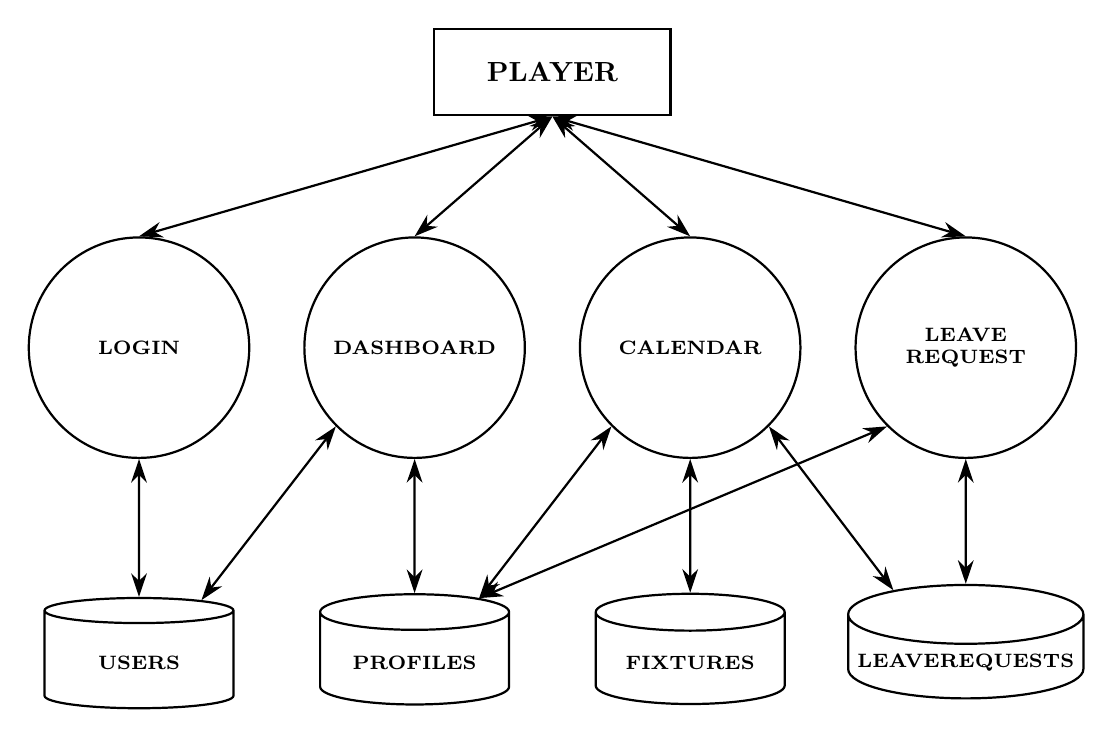
\begin{tikzpicture}[
  entity/.style={rectangle, draw, thick, minimum width=3cm, minimum height=1.1cm, font=\normalsize\bfseries, text centered},
  process/.style={circle, draw, thick, minimum size=2.8cm, font=\scriptsize\bfseries, text width=2.3cm, align=center},
  datastore/.style={cylinder, draw, thick, shape border rotate=90, aspect=0.25, minimum width=2.4cm, minimum height=1.4cm, font=\scriptsize\bfseries, text centered},
  biarr/.style={{Stealth[length=3mm, width=2mm]}-{Stealth[length=3mm, width=2mm]}, thick}
]

\node[entity] (player) at (0, 6) {PLAYER};

\node[process] (p1) at (-5.25, 2.5)  {LOGIN};
\node[process] (p2) at (-1.75, 2.5)  {DASHBOARD};
\node[process] (p3) at (1.75, 2.5)   {CALENDAR};
\node[process] (p4) at (5.25, 2.5)   {LEAVE\\REQUEST};

\node[datastore] (d1) at (-5.25, -1.5)  {USERS};
\node[datastore] (d2) at (-1.75, -1.5)  {PROFILES};
\node[datastore] (d3) at (1.75, -1.5)   {FIXTURES};
\node[datastore] (d4) at (5.25, -1.5)   {LEAVE\\REQUESTS};

\draw[biarr] (player.south) -- (p1.north);
\draw[biarr] (player.south) -- (p2.north);
\draw[biarr] (player.south) -- (p3.north);
\draw[biarr] (player.south) -- (p4.north);

\draw[biarr] (p1.south) -- (d1.north);
\draw[biarr] (p2.south) -- (d2.north);
\draw[biarr] (p3.south) -- (d3.north);
\draw[biarr] (p4.south) -- (d4.north);

\draw[biarr] (p2.south west) -- (d1.north east);
\draw[biarr] (p3.south east) -- (d4.north west);
\draw[biarr] (p3.south west) -- (d2.north east);
\draw[biarr] (p4.south west) -- (d2.north east);

\end{tikzpicture}
\end{document}
